\documentclass{standalone}
\usepackage{tikz}
\usetikzlibrary{patterns, positioning}


\begin{document}
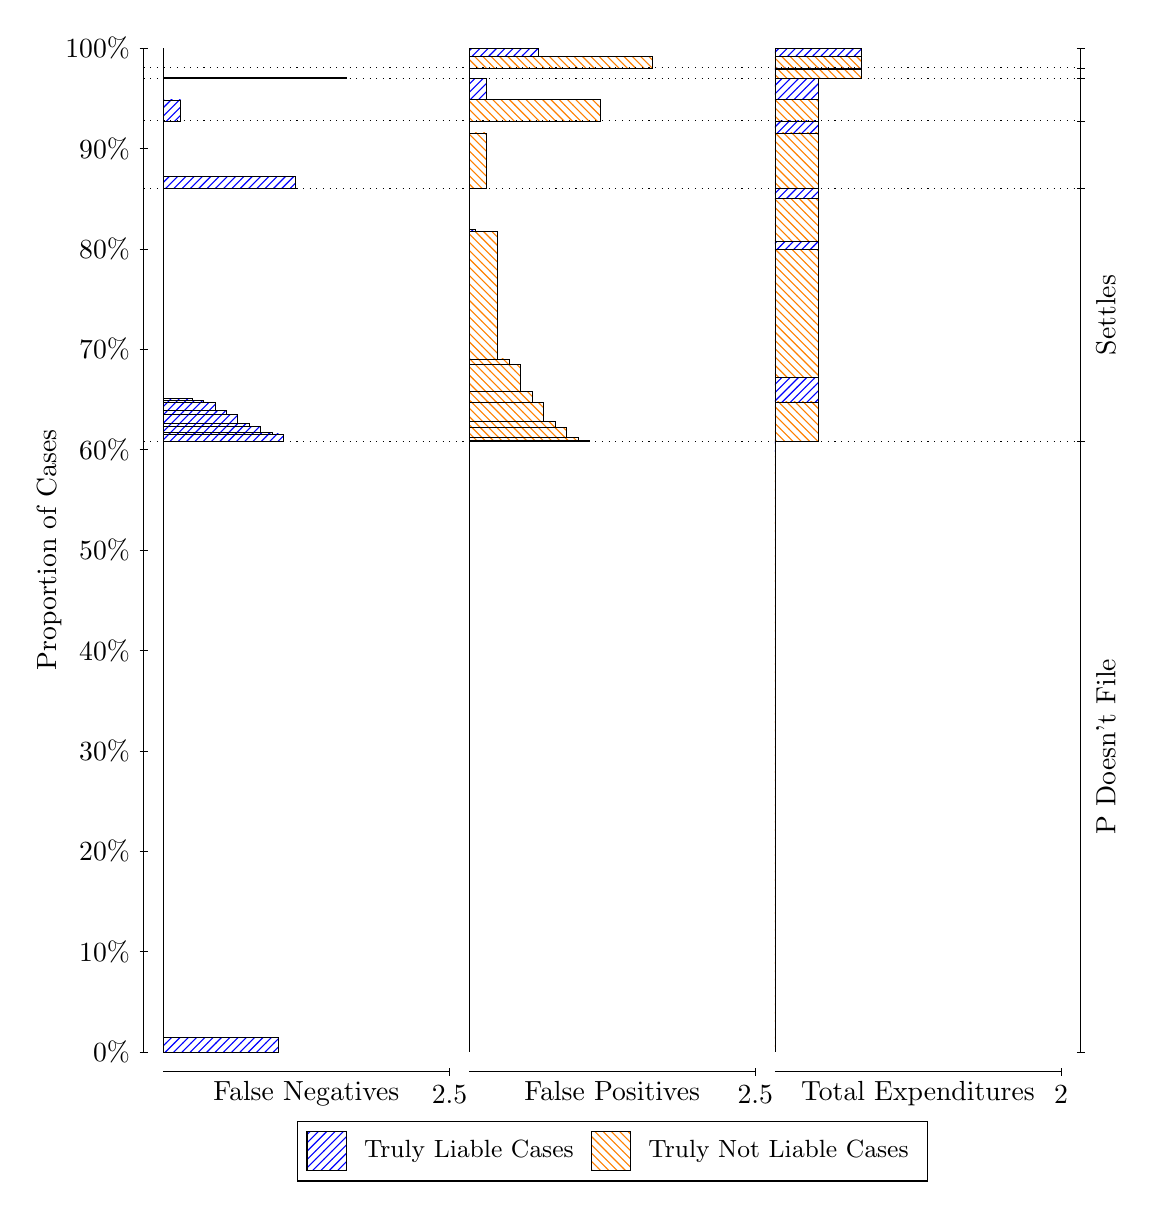
\begin{tikzpicture}
\draw[black, very thin] (1.5,1.75) -- (1.5,14.5);
\node[rotate=90, text=black, anchor=center] at (0.3, 8.125) {Proportion of Cases};
\draw[black, very thin] (1.45,1.75) -- (1.55,1.75);
\node[text=black, anchor=east] at (1.45, 1.75) {0\%};
\draw[black, very thin] (1.45,3.025) -- (1.55,3.025);
\node[text=black, anchor=east] at (1.45, 3.025) {10\%};
\draw[black, very thin] (1.45,4.3) -- (1.55,4.3);
\node[text=black, anchor=east] at (1.45, 4.3) {20\%};
\draw[black, very thin] (1.45,5.575) -- (1.55,5.575);
\node[text=black, anchor=east] at (1.45, 5.575) {30\%};
\draw[black, very thin] (1.45,6.85) -- (1.55,6.85);
\node[text=black, anchor=east] at (1.45, 6.85) {40\%};
\draw[black, very thin] (1.45,8.125) -- (1.55,8.125);
\node[text=black, anchor=east] at (1.45, 8.125) {50\%};
\draw[black, very thin] (1.45,9.4) -- (1.55,9.4);
\node[text=black, anchor=east] at (1.45, 9.4) {60\%};
\draw[black, very thin] (1.45,10.675) -- (1.55,10.675);
\node[text=black, anchor=east] at (1.45, 10.675) {70\%};
\draw[black, very thin] (1.45,11.95) -- (1.55,11.95);
\node[text=black, anchor=east] at (1.45, 11.95) {80\%};
\draw[black, very thin] (1.45,13.225) -- (1.55,13.225);
\node[text=black, anchor=east] at (1.45, 13.225) {90\%};
\draw[black, very thin] (1.45,14.5) -- (1.55,14.5);
\node[text=black, anchor=east] at (1.45, 14.5) {100\%};

\draw[black, very thin] (13.4,1.75) -- (13.4,14.5);
\draw[black, very thin] (13.35,1.75) -- (13.45,1.75);
\node[anchor=west] at (13.35, 1.75) {};
\draw[black, very thin] (13.35,9.5027) -- (13.45,9.5027);
\node[anchor=west] at (13.35, 9.5027) {};
\draw[black, very thin] (13.35,12.718) -- (13.45,12.718);
\node[anchor=west] at (13.35, 12.718) {};
\draw[black, very thin] (13.35,13.575) -- (13.45,13.575);
\node[anchor=west] at (13.35, 13.575) {};
\draw[black, very thin] (13.35,14.113) -- (13.45,14.113);
\node[anchor=west] at (13.35, 14.113) {};
\draw[black, very thin] (13.35,14.248) -- (13.45,14.248);
\node[anchor=west] at (13.35, 14.248) {};
\draw[black, very thin] (13.35,14.5) -- (13.45,14.5);
\node[anchor=west] at (13.35, 14.5) {};

\draw[black, very thin, pattern color=blue, pattern=north east lines] (1.75,1.75) rectangle (3.2033,1.9359);
\draw[black, very thin, pattern color=orange, pattern=north west lines] (1.75,1.9359) rectangle (1.75,9.5027);
\draw[black, very thin, pattern color=blue, pattern=north east lines] (1.75,9.5027) rectangle (3.276,9.6008);
\draw[black, very thin, pattern color=blue, pattern=north east lines] (1.75,9.6008) rectangle (3.1307,9.6157);
\draw[black, very thin, pattern color=blue, pattern=north east lines] (1.75,9.6157) rectangle (2.9853,9.6956);
\draw[black, very thin, pattern color=blue, pattern=north east lines] (1.75,9.6956) rectangle (2.84,9.7339);
\draw[black, very thin, pattern color=blue, pattern=north east lines] (1.75,9.7339) rectangle (2.6947,9.8509);
\draw[black, very thin, pattern color=blue, pattern=north east lines] (1.75,9.8509) rectangle (2.5493,9.8997);
\draw[black, very thin, pattern color=blue, pattern=north east lines] (1.75,9.8997) rectangle (2.404,9.9949);
\draw[black, very thin, pattern color=blue, pattern=north east lines] (1.75,9.9949) rectangle (2.2587,10.027);
\draw[black, very thin, pattern color=blue, pattern=north east lines] (1.75,10.027) rectangle (2.1133,10.048);
\draw[black, very thin, pattern color=orange, pattern=north west lines] (1.75,10.048) rectangle (1.75,12.718);
\draw[black, very thin, pattern color=blue, pattern=north east lines] (1.75,12.718) rectangle (3.4213,12.87);
\draw[black, very thin, pattern color=orange, pattern=north west lines] (1.75,12.87) rectangle (1.75,13.575);
\draw[black, very thin, pattern color=blue, pattern=north east lines] (1.75,13.575) rectangle (1.968,13.842);
\draw[black, very thin, pattern color=orange, pattern=north west lines] (1.75,13.842) rectangle (1.75,14.113);
\draw[black, very thin, pattern color=blue, pattern=north east lines] (1.75,14.113) rectangle (4.0753,14.128);
\draw[black, very thin, pattern color=orange, pattern=north west lines] (1.75,14.128) rectangle (1.75,14.248);
\draw[black, very thin, pattern color=orange, pattern=north west lines] (1.75,14.248) rectangle (1.75,14.389);
\draw[black, very thin, pattern color=blue, pattern=north east lines] (1.75,14.389) rectangle (1.75,14.5);
\draw[black, very thin, pattern color=orange, pattern=north west lines] (5.6333,1.75) rectangle (5.6333,9.3169);
\draw[black, very thin, pattern color=blue, pattern=north east lines] (5.6333,9.3169) rectangle (5.6333,9.5027);
\draw[black, very thin, pattern color=orange, pattern=north west lines] (5.6333,9.5027) rectangle (7.1593,9.5212);
\draw[black, very thin, pattern color=orange, pattern=north west lines] (5.6333,9.5212) rectangle (7.014,9.5599);
\draw[black, very thin, pattern color=orange, pattern=north west lines] (5.6333,9.5599) rectangle (6.8687,9.6794);
\draw[black, very thin, pattern color=orange, pattern=north west lines] (5.6333,9.6794) rectangle (6.7233,9.7563);
\draw[black, very thin, pattern color=orange, pattern=north west lines] (5.6333,9.7563) rectangle (6.578,10.002);
\draw[black, very thin, pattern color=orange, pattern=north west lines] (5.6333,10.002) rectangle (6.4327,10.006);
\draw[black, very thin, pattern color=orange, pattern=north west lines] (5.6333,10.006) rectangle (6.4327,10.143);
\draw[black, very thin, pattern color=orange, pattern=north west lines] (5.6333,10.143) rectangle (6.2873,10.483);
\draw[black, very thin, pattern color=orange, pattern=north west lines] (5.6333,10.483) rectangle (6.142,10.552);
\draw[black, very thin, pattern color=orange, pattern=north west lines] (5.6333,10.552) rectangle (5.9967,12.173);
\draw[black, very thin, pattern color=blue, pattern=north east lines] (5.6333,12.173) rectangle (5.706,12.194);
\draw[black, very thin, pattern color=blue, pattern=north east lines] (5.6333,12.194) rectangle (5.6333,12.718);
\draw[black, very thin, pattern color=orange, pattern=north west lines] (5.6333,12.718) rectangle (5.8513,13.423);
\draw[black, very thin, pattern color=blue, pattern=north east lines] (5.6333,13.423) rectangle (5.6333,13.575);
\draw[black, very thin, pattern color=orange, pattern=north west lines] (5.6333,13.575) rectangle (7.3047,13.846);
\draw[black, very thin, pattern color=blue, pattern=north east lines] (5.6333,13.846) rectangle (5.8513,14.113);
\draw[black, very thin, pattern color=orange, pattern=north west lines] (5.6333,14.113) rectangle (5.6333,14.233);
\draw[black, very thin, pattern color=blue, pattern=north east lines] (5.6333,14.233) rectangle (5.6333,14.248);
\draw[black, very thin, pattern color=orange, pattern=north west lines] (5.6333,14.248) rectangle (7.9587,14.389);
\draw[black, very thin, pattern color=blue, pattern=north east lines] (5.6333,14.389) rectangle (6.5053,14.5);
\draw[black, very thin, pattern color=orange, pattern=north west lines] (9.5167,1.75) rectangle (9.5167,9.3169);
\draw[black, very thin, pattern color=blue, pattern=north east lines] (9.5167,9.3169) rectangle (9.5167,9.5027);
\draw[black, very thin, pattern color=orange, pattern=north west lines] (9.5167,9.5027) rectangle (10.062,10.006);
\draw[black, very thin, pattern color=blue, pattern=north east lines] (9.5167,10.006) rectangle (10.062,10.321);
\draw[black, very thin, pattern color=orange, pattern=north west lines] (9.5167,10.321) rectangle (10.062,11.942);
\draw[black, very thin, pattern color=blue, pattern=north east lines] (9.5167,11.942) rectangle (10.062,12.04);
\draw[black, very thin, pattern color=orange, pattern=north west lines] (9.5167,12.04) rectangle (10.062,12.586);
\draw[black, very thin, pattern color=blue, pattern=north east lines] (9.5167,12.586) rectangle (10.062,12.718);
\draw[black, very thin, pattern color=orange, pattern=north west lines] (9.5167,12.718) rectangle (10.062,13.423);
\draw[black, very thin, pattern color=blue, pattern=north east lines] (9.5167,13.423) rectangle (10.062,13.575);
\draw[black, very thin, pattern color=orange, pattern=north west lines] (9.5167,13.575) rectangle (10.062,13.846);
\draw[black, very thin, pattern color=blue, pattern=north east lines] (9.5167,13.846) rectangle (10.062,14.113);
\draw[black, very thin, pattern color=orange, pattern=north west lines] (9.5167,14.113) rectangle (10.607,14.233);
\draw[black, very thin, pattern color=blue, pattern=north east lines] (9.5167,14.233) rectangle (10.607,14.248);
\draw[black, very thin, pattern color=orange, pattern=north west lines] (9.5167,14.248) rectangle (10.607,14.389);
\draw[black, very thin, pattern color=blue, pattern=north east lines] (9.5167,14.389) rectangle (10.607,14.5);
\draw[black, dotted] (1.5,9.5027) -- (13.4,9.5027);
\draw[black, dotted] (1.5,12.718) -- (13.4,12.718);
\draw[black, dotted] (1.5,13.575) -- (13.4,13.575);
\draw[black, dotted] (1.5,14.113) -- (13.4,14.113);
\draw[black, dotted] (1.5,14.248) -- (13.4,14.248);
\draw[black, very thin] (1.75,1.5) -- (5.3833,1.5);
\node[text=black, anchor=north] at (3.5667, 1.5) {False Negatives};
\draw[black, very thin] (5.3833,1.45) -- (5.3833,1.55);
\node[text=black, anchor=north] at (5.3833, 1.45) {2.5};

\draw[black, very thin] (5.6333,1.5) -- (9.2667,1.5);
\node[text=black, anchor=north] at (7.45, 1.5) {False Positives};
\draw[black, very thin] (9.2667,1.45) -- (9.2667,1.55);
\node[text=black, anchor=north] at (9.2667, 1.45) {2.5};

\draw[black, very thin] (9.5167,1.5) -- (13.15,1.5);
\node[text=black, anchor=north] at (11.333, 1.5) {Total Expenditures};
\draw[black, very thin] (13.15,1.45) -- (13.15,1.55);
\node[text=black, anchor=north] at (13.15, 1.45) {2};

\node[text=black, centered, rotate=90] at (13.72, 5.6264) {P Doesn't File};
\node[text=black, centered, rotate=90] at (13.72, 11.11) {Settles};





\draw (7.449999999999999,1.5) node[draw=none] (baseCoordinate) {};
\begin{scope}[align=center]
        \matrix[scale=0.5, draw=black, below=0.5cm of baseCoordinate, nodes={draw}, column sep=0.1cm]{
            \node[rectangle, draw, minimum width=0.5cm, minimum height=0.5cm, pattern color=blue, pattern=north east lines] {}; &
            \node[draw=none, font=\small, text=black] (B) {Truly Liable Cases}; &
            \node[rectangle, draw, minimum width=0.5cm, minimum height=0.5cm, pattern color=orange, pattern=north west lines] {}; &
            \node[draw=none, font=\small, text=black] (B) {Truly Not Liable Cases}; \\
            };
\end{scope}

\end{tikzpicture}
\end{document}